\documentclass[UTF8,a4paper,zihao=-4]{ctexart}

\usepackage[
  left=2.5cm,right=2.5cm,
  top=2.6cm,bottom=2.6cm,
  headheight=15pt,headsep=22pt,footskip=30pt
]{geometry}
\usepackage{amsmath,amssymb}
\usepackage{booktabs,longtable,tabularx,array,multirow}
\usepackage{graphicx,float}
\usepackage{xcolor}
\usepackage{tikz}
\usetikzlibrary{arrows.meta,positioning,shapes.geometric}
\usepackage{enumitem}
\usepackage{fancyhdr}
\usepackage{hyperref}

\definecolor{accent}{HTML}{176B87}
\definecolor{softblue}{HTML}{EAF4F8}
\definecolor{softgray}{HTML}{F3F4F6}
\hypersetup{colorlinks=true,linkcolor=accent,citecolor=accent,urlcolor=accent,pdfauthor={匿名参赛团队},pdftitle={李萨如图形虚拟实验教学资源设计报告}}
\setlength{\parindent}{2em}
\setlength{\parskip}{0.25em}
\setlist{nosep,leftmargin=2em}
\renewcommand{\arraystretch}{1.25}
\pagestyle{fancy}
\fancyhf{}
\fancyhead[L]{第十二届全国大学生物理实验竞赛（创新）}
\fancyhead[R]{自选题2：教学资源和虚仿}
\fancyfoot[C]{\thepage}

\newcommand{\todoitem}[1]{\textcolor{red!70!black}{【待参赛队补充：#1】}}
\newcommand{\code}[1]{\texttt{#1}}

\begin{document}

\hypersetup{pageanchor=false}
\begin{titlepage}
\thispagestyle{empty}
  \centering
  \vspace*{1.5cm}
  {\zihao{2}\bfseries 第十二届全国大学生物理实验竞赛（创新）\par}
  \vspace{0.8cm}
  {\zihao{3}\bfseries 自选题2：教学资源和虚仿\par}
  \vspace{1.8cm}
  {\zihao{1}\bfseries 李萨如图形虚拟实验室\par}
  \vspace{0.4cm}
  {\zihao{3}相位差、振幅比、频率比与频率失谐的交互式教学资源\par}
  \vfill
  \begin{tabular}{rl}
    作品类别：& 自选题2——教学资源和虚仿\\
    作品形态：& 交互式虚拟实验与智能助教\\
    参赛编号：& \todoitem{由竞赛系统生成后填写}\\
    报告版本：& 竞赛匿名送审稿（草案）\\
    日期：& 2026年\quad 月\quad 日
  \end{tabular}
  \vfill
  {\small 本报告不出现学校名称、指导教师姓名和学生姓名。成员以匿名编号表示。}
\end{titlepage}
\hypersetup{pageanchor=true}

\pagenumbering{Roman}
\section*{摘要}
本作品面向大学物理实验中“正交简谐振动合成”这一兼具抽象性与可观测性的教学难点，开发了李萨如图形交互式虚拟实验室。系统以可验证的解析模型和离散采样为核心，将相位差、振幅比、有理频率比和频率失谐四个实验置于统一界面中，同步显示双通道时域波形、二维轨迹、运动方向、辅助分析曲线和定量读数。用户可改变物理参数、控制形成过程，并导出图像与数据，用于“预测—观察—测量—解释—复核”的探究式学习。

作品同时提供基于本地文献知识库的智能问答，但问答模块与数值仿真核心相互隔离：物理结果由确定性公式和程序计算产生，生成式人工智能不参与修改实验数据。系统采用 Python--Julia 混合编程：Python/Streamlit 负责统一网页、知识检索、问答、安全执行与进程调度，Julia/WGLMakie 负责确定性物理计算和高性能交互图形；两端通过本机回环网页服务在浏览器中组合。作品已封装为 Windows 单文件版本，目标计算机无需预装 Python 和 Julia 环境，强化了安装便利性、维护性与推广价值。报告给出物理模型、软件架构、实现流程、参数范围、验证方案、教学应用、局限性、软硬件要求及学术规范说明。

\noindent\textbf{关键词：}李萨如图形；简谐振动；虚拟实验；Python--Julia 混合编程；交互可视化；智能助教
\clearpage
\tableofcontents
\clearpage
\pagenumbering{arabic}

\section{选题意义与目标定位}

\subsection{教学背景与选题价值}
李萨如图形是正交简谐振动合成的直观表现，也是连接振动方程、示波器工作原理、频率测量和相位测量的重要教学载体\cite{cena2014,doll2007,hogan2019}。它把两路随时间变化的一维信号映射为二维几何轨迹，使学生能够从“波形随时间变化”和“轨迹在平面形成”两种视角认识同一物理过程。相关思想还可迁移到交流电相位比较、模态振动、周期信号辨识和 MEMS 扫描；现代研究表明扫描密度、互质频率和相位漂移会直接影响成像质量\cite{wang2020,birla2020,janin2022}，因此李萨如图形并非孤立的演示现象，而是培养参数化建模与图像判读能力的典型案例。

真实示波器实验具有不可替代的仪器操作价值，现有实验手册和数字示波器拓展项目也证明了 $X$--$Y$ 模式在测频、测相和图像重建中的教学潜力\cite{uestc,tongji,huang2025}。但课堂时间、信号稳定性、触发设置和设备数量会限制学生对参数空间的系统探索。特别是在频率比稍复杂或两路频率存在微小失谐时，轨迹持续演化，学生很难在一次短暂观察中同时记录波形、方向、闭合周期和定量误差。虚拟实验可以提供可重复、可暂停、可逐帧和可导出的观察条件，使学习者在进入真实实验前形成预测，在操作后利用模型复核现象，从而把有限的实体实验时间更多用于接线、调节、测量和误差辨识。

本作品选取相位差、振幅比、有理频率比和频率失谐四条相互关联的探究主线。前两者研究同频条件下的几何性质，第三个模块研究严格周期闭合，第四个模块进一步讨论近似同频时的慢演化。四个模块由简到繁，形成“理想模型—定量规律—边界条件—非理想扩展”的学习序列。

这一序列并非四个彼此独立的动画集合，而是一条连续的概念发展路径。学生先在同频条件下建立“一个参数变化对应一种几何变化”的控制变量意识，再通过有理频率比认识多个时间尺度的公周期，最后进入频率失谐导致的准周期慢演化。前一模块得到的相位、尺度和闭合概念都会在后一模块再次出现，使学习者逐步从识别典型图形过渡到解释任意参数组合。作品因此既可作为短时课堂演示，也可拆分为若干次具有前后依赖关系的探究任务。

\subsection{现有教学中的主要困难}
传统示波器实验能够显示轨迹，却不容易同时呈现两路时域信号、轨迹形成顺序、运动方向和定量关系。常见学习困难及本作品的对应解决方式见表~\ref{tab:liss-problems}。

从认知过程看，学生需要在三个表征层次间不断转换：第一层是两路振动的时间函数，第二层是同一时刻的有序数对 $(x,y)$，第三层是大量有序数对构成的几何轨迹。任一层次被省略，都可能使动态图形退化为需要背诵的图案。因而界面必须保持时间轴、二维坐标和物理参数之间的对应关系，并通过当前点、方向箭头和定量读数降低表征转换负担。

从实验方法看，图形“看起来闭合”并不等于严格周期闭合，图形“看起来相同”也不一定对应唯一相位差。作品需要同时支持定性观察和定量判据，使学生能够用闭合周期、终点误差、椭圆参数和累积相位检验视觉判断，而不是把屏幕截图本身当作结论。

\begin{table}[!htb]
\centering
\caption{教学困难与作品设计响应}
\label{tab:liss-problems}
\begin{tabularx}{\textwidth}{p{3.2cm}X X}
\toprule
教学困难 & 典型表现 & 作品设计响应\\
\midrule
方程与图形脱节 & 能代入公式，却不能说明某一时刻的两路位移如何确定轨迹点 & 同步显示 $x(t)$、$y(t)$、当前采样点和二维运动方向\\
变量作用混淆 & 把振幅比、相位差和频率比对图形的影响混为一谈 & 四个实验模块分离自变量，并提供重置和单变量探究路径\\
只记结论、不知条件 & 机械记忆“相差 $90^\circ$ 是圆”或“叶数等于频率比” & 同时显示适用条件、约分频率比、闭合周期和终点误差\\
静态图难表征慢演化 & 无法解释微小频差为何使图形持续旋转、舒张或收缩 & 显示累积相位和 $T_{\mathrm{shape}}=1/|\Delta f|$，并支持进程控制\\
观察难以复核 & 实验结束后缺少原始轨迹数据，无法进一步拟合与检验 & 导出时间序列和参数，支持独立绘图、残差计算与报告分析\\
\bottomrule
\end{tabularx}
\end{table}

本作品把不可直接观察的相位累积和时间演化映射为同步动画与数值读数，并要求学生每次只改变一个自变量。其目标不是替代真实示波器，而是为真实实验提供可反复使用的认知支架和数据复核工具。

针对上述困难，作品采用“同一参数、三种证据”的呈现策略：时域曲线说明两路信号在何时取何值，二维轨迹说明这些同步取值如何形成几何图案，解析读数则说明图案应满足何种定量规律。三种证据若相互一致，学生的解释才算完整；若不一致，便可进一步检查参数设置、采样、归一化或读图过程。这种设计把错误从单纯的“答案错误”转化为可定位的模型诊断过程。

\subsection{作品定位}
作品严格按“自选题2：教学资源和虚仿”定位，具有以下特征：
\begin{enumerate}
  \item 自主构建正交简谐振动、椭圆几何、闭合周期与相位累积模型；
  \item 允许参数连续或离散调节，输出时域、轨迹和定量分析结果；
  \item 提供完整的使用路径、模型自检、数据导出和单文件部署；
  \item 提供文献检索型智能问答，辅助解释现象、比较方案和分析误差；
  \item 保持数值核心透明，避免“黑箱式生成最终答案”。
\end{enumerate}

作品遵循三项设计原则。第一是\textbf{科学性优先}：所有轨迹和读数均由明确的物理方程计算，图形变化必须能回到参数和公式解释。第二是\textbf{学习过程可见}：不仅展示最终曲线，还展示形成顺序、运动方向、参考波形和派生量。第三是\textbf{虚实互补}：虚拟实验负责扩大可探索范围和提供理想参照，真实实验负责培养仪器使用、信号调节和不确定度分析能力。智能问答仅承担提示、文献解释和拓展讨论，不改变仿真数据。

据此，作品形成三条彼此独立而又可相互核查的数据链：Julia 模型链负责从参数生成确定性轨迹，浏览器交互链负责把状态变化呈现给学习者，智能问答链负责从专题文献和计算工具组织解释。三条链在界面上汇合，但数值来源并不混合。这样的分层既便于教学时说明“图从哪里来、结论凭什么成立”，也便于开发阶段分别测试模型正确性、界面可用性和问答可靠性。

\subsection{适用对象与教学场景}
作品主要面向已学习简谐振动、但尚未系统掌握示波器 $X$--$Y$ 模式的大学低年级学生，也可用于中学物理竞赛拓展和大学物理课堂演示。典型应用包括：
\begin{itemize}
  \item \textbf{实验前预习：}根据给定参数预测图形，完成相位、振幅和频率比的诊断题；
  \item \textbf{课堂讲授：}教师逐步改变单一参数，组织学生用方程解释动态图形；
  \item \textbf{实体实验配套：}把示波器实测图与理想轨迹对照，讨论噪声、通道增益和频率漂移；
  \item \textbf{课后探究：}导出数据，研究闭合误差、相位反演或近有理频率比下的长周期行为；
  \item \textbf{自主答疑：}围绕图形判读、测量步骤和误差来源检索文献并形成可核查解释。
\end{itemize}

在具体实施中，教师可根据课时长度选择不同深度。十分钟演示可只使用相位特殊值和运动方向；一次完整实验课可安排四个控制变量任务及数据导出；开放实验则可加入真实示波器截图、未知信号反演和近有理频率比研究。学生端既可以按照任务单逐步操作，也可以从智能问答中的现象问题进入相应实验模块。因而同一资源能够兼顾教师主导讲授、学生协作探究和个体补偿学习。

\subsection{教学目标}
本作品将教学目标分为知识、能力、科学思维和实验素养四个层次：
\begin{enumerate}
  \item \textbf{知识目标：}掌握正交简谐振动的参数方程，理解相位差、振幅比、频率比和频率失谐的物理含义；
  \item \textbf{能力目标：}能够由参数预测轨迹、由图形反推条件，并使用导出数据完成定量检验；
  \item \textbf{科学思维目标：}形成控制变量、极限情形、量纲检查和模型边界意识，区分“观察到相关性”与“由方程得到因果解释”；
  \item \textbf{实验素养目标：}理解理想仿真与真实仪器之间的差异，能把模型偏差转化为可检验的误差假设。
\end{enumerate}

四类目标之间具有明确的递进关系：知识目标回答“参数与图形有什么关系”，能力目标回答“如何用数据检验这种关系”，科学思维目标回答“结论依赖哪些假设”，实验素养目标则要求把理想结论迁移到真实仪器。教学活动和评价题目均围绕这一递进组织，避免只以能否复述典型相位图形作为学习达成标准。

\subsection{预期学习成果}
完成实验后，学习者应能：
\begin{itemize}
  \item 从两个正交简谐振动写出参数方程并判断典型轨迹；
  \item 区分相位差、振幅比和频率比对图形的不同作用；
  \item 推导并验证有理频率比下的最短闭合周期；
  \item 用 $T_{\mathrm{shape}}=1/|\Delta f|$ 解释频率失谐造成的慢变化；
  \item 依据导出数据进行拟合、残差判断和误差讨论；
  \item 认识仿真模型的适用边界，并设计与真实示波器实验的对照任务。
\end{itemize}

上述成果采用可观察证据评价，而不只依赖主观反馈：预测表用于检查概念理解，导出数据和残差用于检查定量能力，实验前后同构题用于比较学习增益，虚实对照报告用于检查误差分析与模型边界意识。由此形成“预测—操作—记录—解释—复核—迁移”的教学闭环。

\section{物理原理与计算模型}

\subsection{模型边界、坐标约定与统一表达}
李萨如图形是同一时间参数驱动的两个正交简谐运动在平面上的合成轨迹。设横、纵通道分别为
\begin{equation}
  x(t)=A\sin(2\pi f_x t+\varphi_x),\qquad
  y(t)=B\sin(2\pi f_y t+\varphi_y),
  \label{eq:liss-unified}
\end{equation}
其中 $A,B>0$，相位差定义为 $\varphi=\varphi_y-\varphi_x$。模型假定两通道使用同一时钟、坐标轴相互垂直，且一次观察期间幅值、频率与初相保持不变；暂不引入阻尼、非线性、通道串扰和随机噪声。因此，本作品首先呈现可被解析检验的理想关系，再把“真实仪器中的失真来自何处”留作虚实对照任务。二维谐振子的理论与实验研究表明，频率、幅值和相位共同决定轨道的闭合性与几何形态\cite{cena2014,doll2007}。

同频时可令 $\theta=2\pi ft+\varphi_x$，式\eqref{eq:liss-unified}写成线性映射
\begin{equation}
 \begin{bmatrix}x\\y\end{bmatrix}
 =\underbrace{\begin{bmatrix}A&0\\B\cos\varphi&B\sin\varphi\end{bmatrix}}_{\boldsymbol M}
 \begin{bmatrix}\sin\theta\\\cos\theta\end{bmatrix}.
 \label{eq:liss-matrix}
\end{equation}
右端第二个向量在单位圆上运动，故李萨如椭圆本质上是单位圆经矩阵 $\boldsymbol M$ 的线性变换。程序对 $\boldsymbol M$ 作奇异值分解 $\boldsymbol M=\boldsymbol U\boldsymbol\Sigma\boldsymbol V^{\mathsf T}$：两个奇异值 $\sigma_1,\sigma_2$ 就是椭圆长、短半轴，$\boldsymbol U$ 给出主轴方向。这一计算不依赖“从图上估计宽高”，因而能稳定处理椭圆旋转，并能在退化直线附近保持清晰的几何解释。面积也可由行列式立即得到
\begin{equation}
 S=\pi|\det\boldsymbol M|=\pi AB|\sin\varphi|.
 \label{eq:liss-area}
\end{equation}

\subsection{实验一：相位差与椭圆几何}
在 $f_x=f_y=f$ 的条件下，取 $X=x/A$、$Y=y/B$。由
\begin{equation}
 X=\sin\theta,\qquad
 Y=\sin(\theta+\varphi)=\sin\theta\cos\varphi+\cos\theta\sin\varphi
\end{equation}
消去 $\theta$，得到一般的二次曲线方程
\begin{equation}
  X^2+Y^2-2XY\cos\varphi=\sin^2\varphi,
  \label{eq:liss-conic}
\end{equation}
即
\begin{equation}
  \frac{x^2}{A^2}+\frac{y^2}{B^2}
  -2\frac{xy}{AB}\cos\varphi=\sin^2\varphi.
\end{equation}
当 $A=B$ 时，令 $u=(X+Y)/\sqrt2$、$w=(X-Y)/\sqrt2$，式\eqref{eq:liss-conic}化为
\begin{equation}
 (1-\cos\varphi)u^2+(1+\cos\varphi)w^2=\sin^2\varphi.
\end{equation}
因此主轴沿 $y=x$ 或 $y=-x$，归一化短长轴比为
\begin{equation}
 \frac{b}{a}=\sqrt{\frac{1-|\cos\varphi|}{1+|\cos\varphi|}}.
 \label{eq:liss-axis-ratio}
\end{equation}
$\varphi=0^\circ,180^\circ$ 时 $\det\boldsymbol M=0$，椭圆退化为直线；仅当 $A=B$ 且 $\varphi=90^\circ$ 或 $270^\circ$ 时形成圆。示波器测量资料和 MEMS 相位识别研究同样指出，相位是轨迹重建的敏感参数\cite{hogan2019,birla2020}。

静态轨迹无法区分相反的绕行方向，动态量则可以。计算
\begin{equation}
 x\dot y-y\dot x=-AB(2\pi f)\sin\varphi
 \label{eq:liss-direction}
\end{equation}
可知其符号在一个周期内不变：$\sin\varphi=0$ 时往复运动，否则决定顺、逆时针方向。程序同时绘制当前质点与尾迹，并按屏幕坐标约定标注方向，从而把“相同椭圆外形”和“不同相位演化”区分开来。

\subsection{实验二：振幅比、归一化与面积不变量}
保持频率与相位不变而改变 $A,B$ 时，原始轨迹在坐标轴方向上的总跨度为 $2A$、$2B$，但它们通常不是旋转椭圆的主轴长度。归一化
\begin{equation}
  X=\frac{x}{A},\qquad Y=\frac{y}{B}
\end{equation}
后，振幅尺度被剥离，曲线只保留相位信息；原始图与归一化图的差异因此可用于辨别“通道增益改变”和“相位改变”。程序并列给出两种轨迹，并用式\eqref{eq:liss-matrix}的奇异值报告真实半轴，用式\eqref{eq:liss-area}报告面积。面积对 $A$、$B$ 各呈一次比例，对相位呈 $|\sin\varphi|$ 规律；这既是可视化结论，也是检查数值结果的解析不变量。

需要特别区分坐标方向的幅度与椭圆自身的主轴。$2A$ 和 $2B$ 是轨迹在横、纵坐标上的投影跨度，只有在主轴恰与坐标轴重合时才等于椭圆的轴长；一般相位下，椭圆发生旋转，必须由矩阵 $\boldsymbol M$ 的奇异值确定半轴。教学中先让学生从图上读取横纵跨度，再与程序给出的主轴方向和半轴比较，可以直观揭示“外接矩形”和“旋转椭圆”属于不同几何量，避免把示波器通道刻度直接当作主轴读数。

归一化还提供了一个控制变量检验：固定 $\varphi$，成比例改变 $A$ 或 $B$ 时，原始轨迹的尺寸和面积会改变，而归一化轨迹应保持重合；固定 $A,B$ 改变 $\varphi$ 时，两种轨迹的扁率和方向都会随之变化。学生可导出多组数据，分别检验 $S/(AB)=\pi|\sin\varphi|$ 与归一化隐式方程的残差。这样，振幅比实验不再停留于“图形被拉宽或压窄”的视觉描述，而是形成尺度变换、几何量计算和不变量复核相结合的定量任务。

\subsection{实验三：有理频率比与闭合判据}
若 $f_x=mf_0$、$f_y=nf_0$，闭合要求存在最小正数 $T$，使 $f_xT$ 与 $f_yT$ 同时为整数。令 $g=\gcd(m,n)$，$m'=m/g$、$n'=n/g$，则
\begin{equation}
 T_{\mathrm{close}}=\frac{1}{g f_0},\qquad
 f_xT_{\mathrm{close}}=m',\quad f_yT_{\mathrm{close}}=n'.
 \label{eq:liss-close}
\end{equation}
这说明轨迹是否闭合取决于频率比是否为有理数，而不是两个频率数值是否相等。当前程序允许 $m,n=1,\ldots,6$，先自动约分，再以归一化时间 $u=t/T_{\mathrm{close}}\in[0,1]$ 计算
\begin{equation}
 x(u)=\sin(2\pi m'u),\qquad
 y(u)=\sin(2\pi n'u+\varphi).
\end{equation}
这样，一个绘图区间严格对应一个最短闭合周期。程序还计算
\begin{equation}
 d(u)=\sqrt{[x(u)-x(0)]^2+[y(u)-y(0)]^2},
\end{equation}
并以 $d(1)$ 作为端点闭合误差。理论上 $d(1)=0$；实际显示的极小非零值来自浮点三角函数的舍入误差。该判据比“凭叶数判断”更一般，也可自然推广到复杂频率组合\cite{doll2007,barna2020}。

\subsection{实验四：频率失谐与快慢时间尺度}
令 $f_x=f$、$f_y=f+\Delta f$，相对相位为
\begin{equation}
 \Delta\varphi(t)=2\pi\Delta f\,t+\varphi_0,
 \label{eq:liss-detune-phase}
\end{equation}
因而同时存在载波周期 $T_c=1/f$ 和形态周期
\begin{equation}
 T_{\mathrm{shape}}=\frac{1}{|\Delta f|}\quad(\Delta f\ne0).
 \label{eq:liss-shape-period}
\end{equation}
当 $|\Delta f|\ll f$ 时，一个载波周期内相对相位仅改变约 $2\pi\Delta f/f$，轨迹可近似看作由式\eqref{eq:liss-conic}描述的“瞬时椭圆”；经过较长时间，其取向和扁率又随式\eqref{eq:liss-detune-phase}缓慢变化。程序用进度参数定位 $0$ 至 $T_{\mathrm{shape}}$ 的观察时刻，仅绘制该时刻附近一个载波周期的局部轨迹，同时给出未折返的累计相位和映射到 $0^\circ$--$360^\circ$ 的等效相位。$\Delta f$ 的符号控制演化方向，绝对值控制快慢；当 $\Delta f=0$ 时不存在有限形态周期，程序改用两个载波周期作为观察范围。机械振动和谐振扫描研究也表明，微小频漂和相位延迟会造成轨迹的慢旋转或成像失配\cite{birla2020,janin2022,denhartog1956}。

\subsection{离散化、数值误差与模型校验}
连续方程最终以离散点绘制。相位差和振幅比模块在 $u_i=i/(N-1)$ 上取 $N=1001$ 个点；有理频率比模块为提高多叶曲线的分辨率取 $N=1601$；失谐模块在当前时刻之前的一个载波周期内取 $N=1001$。所有通道由同一数组生成，避免横、纵信号错位。动画只改变当前索引或观察时刻，不改变物理方程，因此暂停、拖动和导出所得数据保持一致。

模型通过四类相互独立的量进行校验：一是式\eqref{eq:liss-conic}的代数残差；二是奇异值半轴与式\eqref{eq:liss-axis-ratio}的解析结果；三是数值面积与 $\pi AB|\sin\varphi|$；四是闭合周期终点误差 $d(1)$。特殊点 $\varphi=0^\circ,90^\circ,180^\circ,270^\circ$ 还可作为退化直线、圆和方向翻转的边界测试。应当指出，当前模型验证的是理想正弦合成规律；实体示波器中的采样不同步、直流偏置、增益误差、相位抖动和非正交偏转板会使轨迹偏离上述方程，这些偏离正是后续虚实对照和误差分析的研究对象。

\section{作品总体设计与实现流程}

\subsection{软件架构}
\begin{figure}[!htb]
\centering
\begin{tikzpicture}[
  node distance=6mm and 8mm,
  box/.style={draw=accent,rounded corners,fill=softblue,align=center,minimum height=9mm,text width=27mm,font=\small},
  line/.style={-{Latex[length=2mm]},thick,draw=accent}
]
\node[box] (user) {学习者\\浏览器交互};
\node[box,right=of user] (ui) {Python\\Streamlit 控制层};
\node[box,above right=of ui] (lab) {Julia + WGLMakie\\确定性物理仿真};
\node[box,below right=of ui] (rag) {本地文献检索\\智能问答};
\node[box,right=of lab] (out) {图形、读数\\CSV/PNG};
\node[box,right=of rag] (kb) {PDF知识库\\TF--IDF + BM25};
\draw[line] (user)--(ui);
\draw[line] (ui)--(lab);
\draw[line] (ui)--(rag);
\draw[line] (lab)--(out);
\draw[line] (rag)--(kb);
\draw[line] (kb)--(rag);
\end{tikzpicture}
\caption{Python 控制层与 Julia 仿真层组成的混合架构。仿真数值核心与生成式问答相互隔离。}
\end{figure}

架构采用前端协调、后端分工的方式。Streamlit 负责页面导航、实验嵌入、对话状态和文件上传；Julia 端只接收经过范围校验的实验参数，返回曲线、读数和导出数据；知识库模块负责文献索引与召回，生成模型只在获得检索上下文后组织自然语言。实验模块即使在问答服务不可用时仍可独立工作，问答模块也不能直接修改 Julia 的真实参数或结果。这种松耦合结构降低了某一服务异常对整个作品的影响，并使单元测试能够针对不同模块分别进行。

系统内部把数据进一步划分为三类：实验参数与轨迹属于确定性数据，检索片段与来源元数据属于证据数据，对话文本属于解释性数据。确定性数据只能由物理模型和参数校验流程产生；证据数据保留文献名、页码或主题等追溯信息；解释性数据可以引用前两类内容，却不能反向覆盖它们。界面虽然把三类信息显示在同一页面，数据所有权仍保持分离，因此教师能够明确判断某个结论来自解析模型、检索材料还是语言组织。

各模块之间使用小而稳定的接口交换状态，而不共享隐含的全局变量。实验端的基本接口是模式、参数、播放进度与导出结果，问答端的基本接口是问题、图片、检索上下文和确定性工具输出。若某一接口收到越界值、缺失资源或尚未就绪的服务状态，控制层先生成可理解的错误提示，并保留其他模块的可用功能。这种接口约束既便于构造边界测试，也使后续替换图形库、检索算法或模型服务时不必重写物理计算核心。

\subsection{Python--Julia 混合编程与进程协同}
本作品的混合编程不是把两种语言机械拼接，也不是在 Python 进程内直接加载 Julia 动态库，而是采用\textbf{进程级解耦、网页级组合}的工程结构。Python 作为控制层，负责启动 Streamlit 主界面、组织智能问答与专题检索、管理上传文件和对话状态，并负责发现可用端口、启动 Julia 子进程、写入日志和判断服务是否就绪；Julia 作为计算与可视化层，依据解析模型生成离散信号和李萨如轨迹，再由 WGLMakie 与 Bonito 建立可观察状态，将控件变化、曲线更新和 WebGL 图形持续发送到浏览器\cite{software}。这种分工分别利用了 Python 在人工智能生态、文本处理和应用编排方面的优势，以及 Julia 在数值表达、科学计算和交互式科学可视化方面的优势。

\begin{table}[!htb]
\centering
\caption{Python 与 Julia 在李萨如实验中的职责边界}
\begin{tabularx}{\textwidth}{p{2.5cm}XX}
\toprule
层次 & Python/Streamlit & Julia/WGLMakie\\
\midrule
核心职责 & 统一入口、知识库检索、智能问答、多模态输入、受限 Python 绘图与进程管理 & 四个实验的方程计算、离散采样、派生量计算、交互控件和 WebGL 绘图\\
状态管理 & 保存页面、对话、上传文件、运行日志及 Julia 服务状态 & 保存实验模式、物理参数、播放索引、轨迹数组和可观察变量\\
交互接口 & 生成 Julia 本机地址并以网页组件嵌入，不转发每一次滑块操作 & 通过 Bonito 网页会话直接响应实验控件，并更新浏览器中的图形与读数\\
输出与验证 & 展示问答、错误提示和实验容器，管理 Python 绘图产物 & 输出 CSV/PNG、解析量和模型自检结果，供 Python 侧页面及外部工具复核\\
\bottomrule
\end{tabularx}
\end{table}

\begin{sloppypar}
启动时，Python 先把主网页和 Julia 网页实验分配到本机回环地址的不同端口，再通过环境变量把主机名、端口和日志目录传给 Julia 运行时。Julia 子进程启动后，Python 使用轻量 TCP 连接检查监听端口是否建立，而不反复请求计算量较大的 WGLMakie 根页面；端口就绪后，Streamlit 组件中的内嵌框架才加载 Julia 页面。学生在实验框架内移动滑块时，事件由浏览器直接交给 Julia/Bonito 会话，Python 无需在两种语言之间逐点复制大数组，因此动画更新链路短、职责清晰。CSV 和 PNG 则作为可移植成果接口，使 Julia 结果能够被 Python、电子表格或其他软件再次验证。
\end{sloppypar}

进程隔离也构成可靠性与安全边界。Julia 初始化失败或超过等待时间时，Python 主页面仍可显示明确状态、日志位置并保留智能问答；问答服务不可用时，Julia 四个确定性实验仍可独立运行。智能问答中由用户确认的 Python 绘图代码在另一套黑名单、独立输出目录和超时机制下执行，不能借由混合编程接口改写 Julia 实验状态。发布阶段再由 PyInstaller 封装 Python 应用，由 PackageCompiler 生成携带 Julia 运行时、WGLMakie 依赖和着色器资源的独立程序，两部分随同一启动器释放并协同启动，从而做到目标机无需预装两种开发环境。

\subsection{实现流程}
每次参数变化均执行下列流程：
\begin{enumerate}
  \item 读取当前实验模式及参数，进行范围约束和边界检查；
  \item 根据解析模型生成统一时间网格和离散信号；
  \item 计算轨迹、几何量、闭合误差或相位累积等派生量；
  \item 通过可观察变量更新时域图、轨迹图、辅助图和读数；
  \item 播放时只改变进程索引，保持理论模型与完整参考曲线不变；
  \item 导出时写入模式、参数和 $t,x,y$ 数据，便于复算与绘图。
\end{enumerate}

程序把“完整参考曲线”和“当前播放状态”分开保存。参数变化时重新计算完整数据，播放时只移动索引并更新高亮部分，因此动画速度不会改变轨迹的物理周期，暂停或拖动也不会重新引入随机状态。导出文件同时写入实验模式、全部参数和数据列名称，使同一结果能够在表格软件、Python 或其他工具中复绘。由此，屏幕动画不是一次性视觉效果，而是解析模型的一种可追溯呈现。

范围约束不仅用于防止界面报错，也承担模型条件提示功能。例如，相位输入统一换算为弧度后再参与计算，频率和振幅必须为正，有理频率比在生成时间网格前先约分，$\Delta f=0$ 则进入不存在有限形态周期的专门分支。程序对这些边界情况给出明确读数，而不通过添加很小的非零数掩盖奇点。这样既可避免数值实现悄然改变物理问题，也能让学生理解公式中的定义域和分段条件。

为了保证一次操作可以复核，界面读数、CSV 数据和辅助图均由同一轮计算结果生成，避免不同组件各自重复计算而产生细微差异。测试时可从任一输出反查输入参数，并用解析公式独立计算面积、闭合周期或形态周期；若结果不一致，则按“参数解析—时间网格—派生量—绘图映射—文件导出”的顺序定位问题。该流程把交互程序转化为具有输入、算法、输出和校验依据的实验系统。

\subsection{界面与交互}
\begin{figure}[!htb]
  \centering
  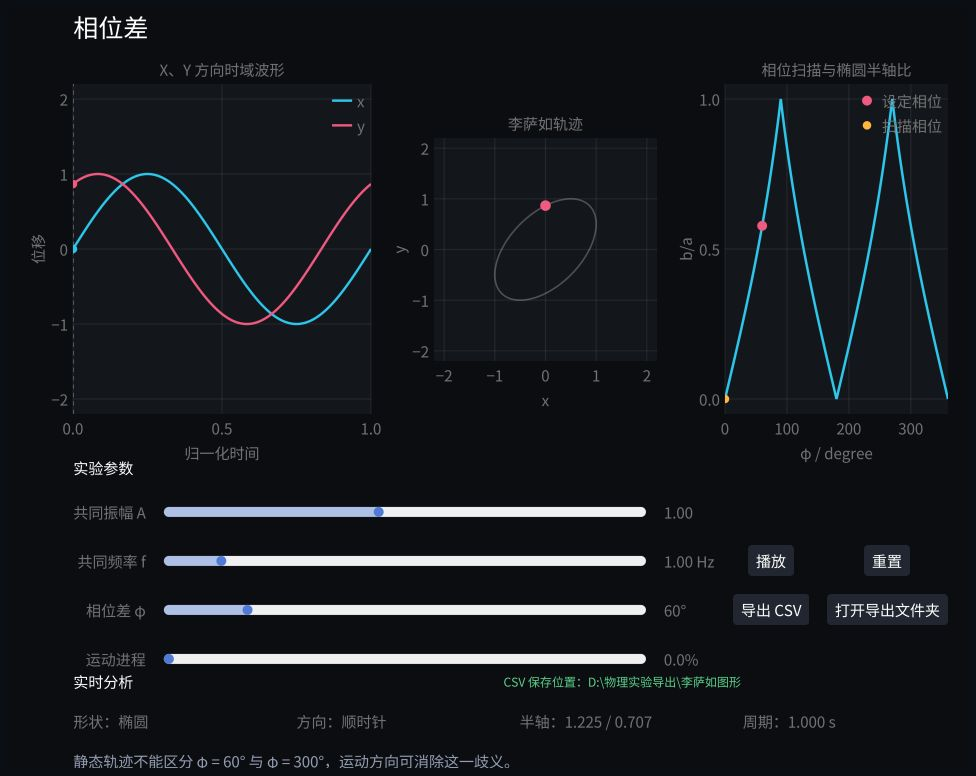
\includegraphics[width=0.98\textwidth]{assets/lissajous_demo_interface.png}
  \caption{李萨如图形综合可视化界面示例。左、中、右区域分别对应时域信号、轨迹形成和定量辅助图。}
\end{figure}

系统将“演示实验”和“智能问答”置于同一助教网页。实验页面由 WGLMakie 在浏览器内渲染，无需额外打开独立窗口；首次加载完成后可切换四个实验页面。问答页面支持文本问题和实验截图，并可对回答中明确选择的 Python 可视化代码进行安全检查后执行。

界面采用“参数在上、证据居中、结论在侧”的组织逻辑。常用控制项保持固定位置，四个模块共享重置、播放、进度和导出操作，降低模块切换带来的额外学习成本；与当前任务无关的控件则被隐藏，避免一次暴露过多变量。颜色和线型不仅用于美观，还承担区分横纵通道、完整轨迹与当前轨迹、理论值与计算值的编码功能。关键数值同时以文本显示，保证学习者即使不依赖颜色也能完成判断。

\section{智能问答特色设计}

\subsection{面向实验学习的功能定位}
本作品没有把通用聊天模型简单嵌入网页，而是围绕李萨如实验建立“现象观察—文献检索—物理推导—确定性计算—可视化验证”的专题助教。它主要解决三类教学需求：一是学生观察到图形后能够立即追问“为什么”；二是把历史文献、示波器测量、机械振动和工程扫描等分散材料组织到当前问题附近；三是把自然语言解释重新连接到可计算参数和可操作实验。智能问答因此不是实验结果的生成器，而是贯穿预习、操作和讨论阶段的认知支架。

与普通搜索或通用对话相比，本助教的特色体现在：问题语境限定于李萨如图形及其拓展应用；回答优先使用项目内经过整理的专题资料；涉及具体频率和相位时调用自研确定性工具；允许上传轨迹、示波器截图和装置照片；当模型服务不可用时仍能退化为本地检索回答。该设计既保留生成式问答的自然交互，也为物理结论设置文献和计算两道约束。

在教学流程中，问答并不只位于实验结束后的“答疑”环节。预习阶段可以要求学生先询问概念但暂不查看完整答案，再写出图形预测；操作阶段可把异常轨迹截图作为追问材料；总结阶段则要求学生比较助教解释、解析公式和导出数据是否一致。通过这种安排，智能问答由答案提供者转化为提出假设、寻找依据和修正解释的工具，学生仍需对最终结论承担推理责任。

\subsection{与校内大学物理智能助教平台的关系}
本实验是学校内部运行的大学物理智能助教平台的专题组成部分，而不是孤立开发的单次演示。校内版本部署在学校服务器上，由统一入口向学生提供课程问答、知识检索、图片理解、学习记录和专题实验服务。校内智能体仅运行学校服务器上的本地模型，不调用外部模型服务；本地模型负责生成与图片理解，本地文献库负责提供课程依据，二者共同构成完全在校内运行的问答链路。

本报告所述的平台关系仅限于统一入口、本地模型推理、文献检索和专题实验的校内部署。李萨如专题的知识范围由本项目整理的专题文献、自研物理模型、实验说明和测试材料构成；其他单位建设的课程知识库、讲义、教案或可视化成果不属于本作品，也不作为本报告的项目成果进行陈述。

平台为专题模块提供通用的网页入口、运行管理和本地推理能力，专题模块则保持物理模型、知识库和实验数据的独立边界。学生围绕轨迹判读、相位测量、频率比和误差分析提出问题时，系统只调用与本专题相关的资料和确定性工具。这样的边界既便于校内部署和维护，也能清楚区分平台公共能力与本竞赛作品的具体贡献。

\begin{table}[!htb]
\centering
\caption{校内平台与本竞赛专题模块的关系}
\begin{tabularx}{\textwidth}{p{3.0cm}X X}
\toprule
层次 & 主要内容 & 在本作品中的作用\\
\midrule
校内平台公共层 & 学校服务器、统一问答入口、校内本地模型与运行管理 & 为专题模块提供校内运行环境和通用交互能力\\
李萨如专题层 & 历史与现代文献、混合检索、相位/频率确定性计算、多模态提示词 & 将通用助教约束到具体物理问题\\
虚拟实验层 & 四个 Julia/WGLMakie 实验、参数控制、读数与数据导出 & 用可复算实验检验问答中的解释\\
竞赛单文件版 & 封装专题前端、知识库与实验运行时 & 便于脱离校内服务器独立演示；模型能力按现场配置运行\\
\bottomrule
\end{tabularx}
\end{table}

\subsection{智能问答界面与交互链路}
\begin{figure}[!htb]
  \centering
  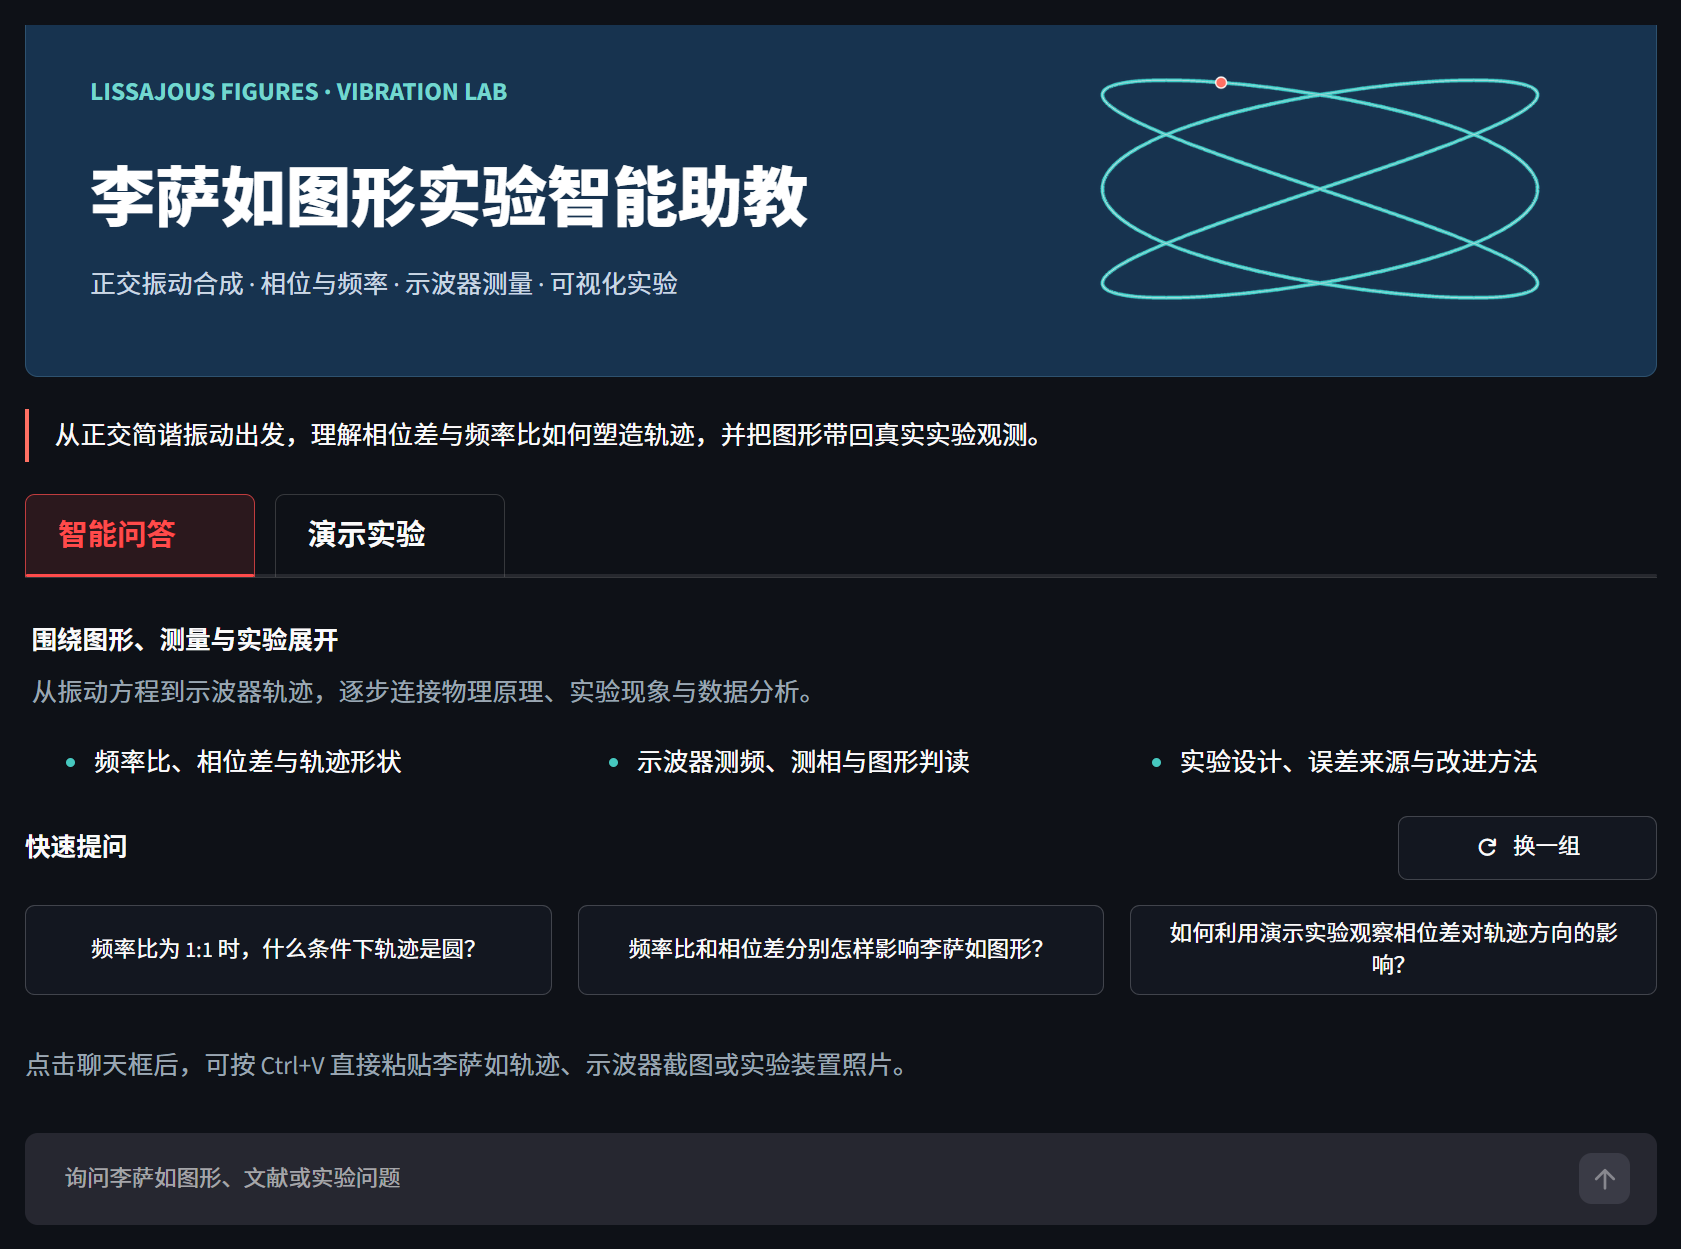
\includegraphics[width=0.98\textwidth]{assets/lissajous_qa_interface_real.png}
  \caption{李萨如图形实验智能助教的真实运行界面。图中展示智能问答入口、专题说明、快速提问与图片粘贴提示。}
\end{figure}

学习者可以直接点击随机生成的三个“快速提问”，也可以输入文字或同时上传多张图片。系统先从本地知识库检索最多 6 条相关材料，再将问题、检索上下文、必要的历史对话和图片交给模型组织回答。回答以流式方式显示；若回答含 Python 绘图代码，界面只提供候选代码和“运行”入口，不自动执行。执行前必须经过危险语句黑名单检查，并在独立输出目录内运行，达到超时上限即终止。该设计把“文献依据—模型解释—数值复核”分开：问答用于启发和解释，轨迹与定量结果仍由确定性实验模型给出。

快速提问并非固定题库的简单展示，而是为初次使用者提供问题范式：原因型问题要求从方程解释现象，方法型问题要求说明测量步骤，误差型问题要求识别模型与仪器的差异。进入连续对话后，系统保留有限轮次上下文以支持指代和参数延续，同时限制历史长度，避免早期无关内容持续影响当前回答。页面还对上传格式、文件大小、模型状态和代码运行状态给出明确反馈，使学生知道系统当前获得了哪些信息、哪些能力可用。

\subsection{专题知识库与混合检索}
知识库由项目中的经典文献、现代研究资料和自研实验说明构建，内容从十九世纪振动曲线与驻波研究延伸到示波器教学、二维谐振子和 MEMS 扫描\cite{cena2014,hogan2019,wang2020,birla2020,huang2025,terquem1878,melde1860}。导入阶段执行 PDF 分页提取、文本清洗、重叠切块，并保存文献名、页码、年份、语言和主题等元数据。对于 Melde 1860 年扫描专篇，项目另行建立逐页德文 OCR 文字层；扫描质量不足的页面记录在提取报告中，不用猜测文字填补空缺。

检索同时使用字符级 TF--IDF 和 BM25，以兼顾中文术语、符号写法与关键词精确匹配。在安装可选稠密向量索引时，综合得分为
\begin{equation}
R=0.48R_{\mathrm{dense}}+0.34R_{\mathrm{TFIDF}}+0.18R_{\mathrm{BM25}}+B_{\mathrm{topic}},
\end{equation}
未安装稠密索引时使用
\begin{equation}
R=0.68R_{\mathrm{TFIDF}}+0.32R_{\mathrm{BM25}}+B_{\mathrm{topic}}.
\end{equation}
程序根据“相位差、互质频率、示波器、机械摆、历史、扫描”等关键词进行查询扩展和主题识别。候选片段低于本轮最高分的 $55\%$ 时被舍弃；同一来源默认只保留一条，以减少单篇文献重复占据上下文。每轮最多选取 6 个来源，拼接上下文不超过约 6200 个字符。联网搜索最多补充 4 条摘要，但与本地原始文献冲突时优先采用原始文献，并要求回答表达不确定性。

字符级 TF--IDF 适合处理中文连续文本、公式附近的短术语以及 $f_x:f_y$ 等符号差异，BM25 则能突出多次出现的核心关键词；两者结合可降低单一检索方法对分词质量的依赖。主题加分只用于把候选结果向当前实验语境轻度偏置，不能把原本不相关的片段提升为依据。检索日志保留查询扩展词、候选得分和来源元数据，便于开发者复查“没有答好”究竟源于文献未导入、检索未命中，还是生成阶段理解错误。

\begin{figure}[!htb]
\centering
\begin{tikzpicture}[
  node distance=6mm and 8mm,
  box/.style={draw=accent,rounded corners,fill=softblue,align=center,minimum height=10mm,text width=29mm,font=\small},
  line/.style={-{Latex[length=2mm]},thick,draw=accent}
]
\node[box] (q) {文字问题、实验图片};
\node[box,right=of q] (expand) {查询扩展、主题识别};
\node[box,right=of expand] (retrieve) {混合检索、来源去重};
\node[box,below=of retrieve] (context) {文献、对话、图片与联网摘要};
\node[box,left=of context] (tool) {频率比、周期、形状与面积计算};
\node[box,left=of tool] (answer) {流式回答或离线检索回退};
\draw[line] (q)--(expand);
\draw[line] (expand)--(retrieve);
\draw[line] (retrieve)--(context);
\draw[line] (context)--(tool);
\draw[line] (tool)--(answer);
\draw[line,dashed] (q.south) |- (tool.west);
\end{tikzpicture}
\caption{李萨如专题问答的数据链路。虚线表示含明确数值参数的问题可触发确定性计算。}
\end{figure}

\subsection{多模态追问与确定性计算}
问答入口接受 PNG、JPG、JPEG 和 WebP 图片，单个上传文件上限为 10 MB。学生可以粘贴李萨如轨迹、双通道示波器画面或装置照片，请助教描述可辨认特征、提出测量步骤并指出信息不足之处。系统保留最近 6 条用户/助教消息，使“这条曲线为何没有闭合”“如果把 $f_y$ 再提高一点会怎样”等连续追问无需反复描述背景。对于模糊图像、缺失刻度或无法确认的装置状态，系统提示词要求明确说明不能可靠读取的部分，不猜测数值。

当问题中出现 $f_x,f_y$、相位差和振幅等明确参数时，程序解析参数并调用自研计算函数，输出约分频率比、闭合判断、最短闭合周期、同频轨迹类型及椭圆面积。该结果作为“确定性计算工具输出”加入回答上下文，模型被要求优先采用，不得用语言模型心算覆盖。回答还可以建议打开相应 Julia 实验，用相同参数进行可视化复核，从而形成自然语言、数值工具和实验页面之间的闭环。

多模态分析强调“可见事实”和“物理推断”的分离。例如，图片中可以直接辨认轨迹是否近似闭合、是否具有某种对称性，却不能在缺少刻度和时间方向时唯一确定振幅、频率或相位。助教需要先列出可观察特征，再说明推断所需的附加信息，最后给出可操作的补测建议。该回答结构既减少对图片的过度解读，也训练学生区分观测、解释和结论三个层次。

\subsection{可选择、受限制的 Python 可视化}
助教能够在回答中给出用于教学绘图的数据处理代码，但代码不会随回答自动执行。学习者必须主动点击运行，系统随后进行正则规则和抽象语法树两级检查。只允许导入 Matplotlib、NumPy、SciPy 和 Pillow；文件读写、动态执行、进程调用、网络访问、环境变量、Streamlit 密钥及敏感运行时属性均被阻止。每次运行创建唯一目录，只传入绘图所需的最小环境变量，默认 60 s 超时，自动收集 PNG、GIF 或视频结果，并仅保留最近 25 个运行目录。

上述机制降低了教学代码误操作和密钥泄露风险，但它不是操作系统级沙箱。报告和界面因此明确要求只运行可信代码；在公共机房部署时还应关闭代码执行或增加容器/低权限账户隔离。这一边界说明是可信设计的一部分，而不是把安全检查描述为绝对防护。

受限代码执行的教学价值在于允许学生对导出数据进行二次表达，例如绘制闭合误差随采样点数的变化、比较不同相位下的面积，或验证归一化前后的轨迹。系统只收集绘图产物而不允许任意文件和网络操作，目的不是提供通用编程环境，而是在明确边界内完成“数据—图形—解释”的短链路任务。教师也可完全关闭该功能而不影响四个 Julia 实验和知识库检索。

\subsection{回答约束、降级机制与质量评价}
系统提示词要求回答区分“文献直接说明”“公式推导”和“教学建议”，不得编造作者、页码、公式或实验数据；多篇资料观点不一致时分别陈述。生成参数采用较低随机性，内容流式显示。若模型接口未配置、鉴权失败或服务中断，系统不会终止整个助教，而是返回确定性计算结果和本地高相关片段，使核心检索能力仍可使用。

项目自带 10 道检索评估题，覆盖基础理论、示波器与相位测量、历史与经典理论、机械振动、数学动力学和 MEMS 扫描。2026 年 8 月 7 日在当前索引上运行评估脚本，10 道题的前 5 条结果均包含预设主题，主题命中率为 $10/10=100\%$。该指标只验证“是否找到相关主题”，不能等同于最终回答完全正确。提交前还需按表~\ref{tab:liss-rag-eval} 完成回答级和教学级评测。

\begin{table}[!htb]
\centering
\caption{智能问答评价框架}
\label{tab:liss-rag-eval}
\begin{tabularx}{\textwidth}{p{3.1cm}p{4.0cm}X}
\toprule
评价维度 & 方法 & 当前状态/提交前证据\\
\midrule
检索主题命中 & 10 道跨主题问题，检查前 5 条是否含目标主题 & 当前版本 $100\%$，可由 \texttt{evaluate.py} 复现\\
物理正确性 & 教师按公式、条件、单位和数量级盲评回答 & \todoitem{补充评分量表、样本数和正确率}\\
依据一致性 & 核查回答是否超出检索片段或把推导冒充文献事实 & \todoitem{补充人工核查结果}\\
图像分析可靠性 & 使用清晰、模糊、缺刻度三组轨迹/示波器图片测试 & \todoitem{补充识别与拒答案例}\\
安全拦截 & 分别测试允许绘图和文件、网络、密钥、进程等危险代码 & 已有自动化单元测试；\todoitem{补充最终测试记录}\\
教学效果 & 比较有/无助教条件下解释题、迁移题和任务完成时间 & \todoitem{补充真实教学数据}\\
\bottomrule
\end{tabularx}
\end{table}

当前版本默认不在每条回答后展示来源列表，来源只作为内部约束保存。为进一步提高可核查性，后续计划增加可展开的“依据卡片”，显示文献题名、页码、相关片段和检索类型，并允许教师关闭联网补充、只使用指定知识库完成考核。

回答质量将采用“结论正确、条件完整、依据一致、计算可复核、教学表达清楚”五项指标分别评分，而不使用单一的总体好坏判断。对于同一道题，可同时保存纯检索回答、模型回答和教师参考答案，比较不同链路在哪些知识点上出现偏差。若回答涉及图像，还需单独记录系统是否正确拒绝读取模糊刻度。这样能够把模型评价转化为可重复的测试集和错误分类，而不是依赖少数演示案例。

\section{使用方法与参数范围}

\subsection{基本操作}
\begin{enumerate}
  \item 双击单文件程序，等待助教网页自动打开；
  \item 进入“演示实验”，选择相位差、振幅比、有理频率比或频率失谐；
  \item 点击“重置”建立基准状态，仅改变一个自变量；
  \item 拖动进程或点击“播放”，观察波形、轨迹和辅助量同步变化；
  \item 记录预测、程序结果和解释，必要时导出数据继续分析；
  \item 在“智能问答”中提出原理、误差和拓展问题，但以实验数据和物理推导作为结论依据。
\end{enumerate}

建议的标准学习记录包含四栏：“改变前预测”“界面观察”“导出数据复算”“最终解释”。学生不得只提交截图，而应注明实验模式、参数、观察时刻和所用判据。若使用智能问答，还需写明采用了哪条建议、如何由公式或数据验证。这样的记录格式能把操作过程转化为可评价证据，也便于教师发现学生是在参数理解、读图还是计算环节遇到困难。

一次完整操作宜按“基准值—特殊值—一般值”展开。学生先用重置状态确认坐标、通道和播放方向，再考察直线、圆、互质频率比等可以直接预测的特殊情形，最后选择一般参数检验结论能否迁移。若界面结果与预测不一致，应依次检查是否改变了多个变量、观察窗口是否覆盖完整周期、频率比是否已经约分以及读数使用的是投影跨度还是主轴长度；完成这些检查后再向智能问答求助。该顺序能够把软件操作转化为诊断过程，避免通过反复拖动滑块偶然寻找“好看的图形”。

\subsection{当前网页实验参数范围}
\begin{longtable}{p{3.2cm}p{3.0cm}p{3.6cm}p{4.2cm}}
\toprule
模式 & 参数 & 范围/步长 & 主要观察量\\
\midrule
\endfirsthead
\toprule
模式 & 参数 & 范围/步长 & 主要观察量\\
\midrule
\endhead
相位差 & $A$；$f$；$\varphi$ & $0.20$--$2.00$，步长$0.05$；$0.5$--$5.0$ Hz，步长$0.1$ Hz；$0^\circ$--$360^\circ$，步长$1^\circ$ & 形状、方向、长短半轴、周期、隐式方程残差\\
振幅比 & $A,B$；$\varphi$ & $A,B=0.20$--$2.00$，步长$0.05$；$0^\circ$--$360^\circ$ & $B/A$、宽、高、面积、归一化轨迹\\
有理频率比 & $f_0$；$m,n$；$\varphi$ & $0.5$--$5.0$ Hz；$m,n=1$--$6$；$0^\circ$--$360^\circ$ & 约分频率比、$f_x,f_y$、$T_{\mathrm{close}}$、终点误差\\
频率失谐 & $A$；$f$；$\Delta f$；$\varphi_0$ & $0.20$--$2.00$；$0.5$--$5.0$ Hz；$-0.40$--$0.40$ Hz，步长$0.01$ Hz；$0^\circ$--$360^\circ$ & $T_{\mathrm{shape}}$、累积相位、等效相位、演化方向\\
全部模式 & 进程 & $0$--$100\%$ & 轨迹形成顺序和当前状态\\
\bottomrule
\end{longtable}
相位、振幅和失谐模式内部采用1001个采样点，有理频率比模式采用1601个采样点。上述范围来自当前程序实现；若参赛版调整参数，应同步更新本表和使用视频。

表中范围是为保证课堂操作稳定、图形变化清晰而设置的教学范围，并不代表真实示波器或信号源的硬件极限。参数边界本身也可成为探究对象：接近 $\varphi=0^\circ$ 时观察椭圆退化，令 $m,n$ 取共同因子检验自动约分，在 $\Delta f$ 接近零时比较载波周期与形态周期。教师应鼓励学生先研究边界和特殊值，再进入一般参数，以便用极限情形检查程序结果。

\section{结果的物理意义、有效性与验证}

\subsection{可复算的理论样例}
\begin{table}[!htb]
\centering
\begin{tabularx}{\textwidth}{p{3.1cm}p{4.1cm}X}
\toprule
验证任务 & 参数 & 理论预期\\
\midrule
相位特殊值 & $A=1, f=1$ Hz，$\varphi=0^\circ,90^\circ,180^\circ$ & 依次得到正斜直线、圆和负斜直线；周期均为1 s\\
振幅与面积 & $A=1,B=0.65,\varphi=60^\circ$ & 宽约2、高约1.30，面积 $S=\pi\times1\times0.65\times\sin60^\circ\approx1.768$\\
频率比闭合 & $f_0=1$ Hz，$m:n=2:3$ & 最短闭合周期1 s，完整周期末 $d(t)$ 回到数值零点\\
未约分输入 & $f_0=1$ Hz，$m:n=2:4$ & 约分为$1:2$，最短闭合周期$0.5$ s\\
频率失谐 & $f=1$ Hz，$\Delta f=0.05$ Hz & 形态变化周期为20 s；$\Delta f$ 变为$-0.05$ Hz时周期不变而方向反转\\
\bottomrule
\end{tabularx}
\caption{程序结果应满足的解析检验。}
\end{table}

程序提供模型自检和界面冒烟测试。提交前应在最终单文件版本上重新执行并记录测试日期、操作系统、浏览器及结果：\todoitem{填写最终测试矩阵、通过率和异常处理记录}。

除解析样例外，还应采用参数扫描进行一致性验证。例如，在 $0^\circ$--$360^\circ$ 范围内检查面积关于 $180^\circ$ 的对称性，在所有 $m,n=1,\ldots,6$ 组合上检查终点误差，在正负成对的 $\Delta f$ 上检查形态周期相等而演化方向相反。测试时既记录是否通过，也记录最大残差和出现位置，从而区分浮点舍入、绘图分辨率与模型错误。最终单文件版还需重复这些测试，以验证封装没有改变资源路径或数值行为。

验证结果应按层次解释，而不能只报告“图形一致”。第一层检查解析量是否满足公式和量纲，第二层检查离散数组的首末点、采样间隔与极值，第三层检查浏览器图形是否正确映射同一数组，第四层检查导出文件能否在独立工具中复绘。数值容差应依据浮点舍入和采样分辨率预先设定，并分别记录绝对误差与相对误差；退化直线或理论值接近零时不宜只使用相对误差。只有四个层次相互一致，才能说明从物理模型到页面输出的完整链路通过验证。

\subsection{教学有效性评价方案}
程序正确不等同于教学有效。拟采用前测/后测与操作任务结合的方式：
\begin{enumerate}
  \item 前测：判断典型图形、解释频率比和相位二义性；
  \item 干预：完成四个单变量探究任务并提交导出数据；
  \item 后测：解释新参数组合，设计真实示波器验证方案；
  \item 记录完成时间、正确率、错误类型和主观认知负荷；
  \item 与传统静态图片或教师演示组比较。
\end{enumerate}
\todoitem{填写样本量、分组方法、量表、统计方法和真实结果；未实测前不得宣称教学效果显著。}

评价题应覆盖记忆、解释和迁移三个层次。前后测可采用不同数值但同一知识结构的平行题，避免学生因记住原题而产生虚假增益；操作任务则用屏幕录制或事件日志分析重置、改单变量、查看读数和导出数据的顺序。除总正确率外，还应编码“把振幅当频率”“忽略相位方向”“以外观代替闭合判据”等典型错误。若样本量允许，可报告效应量和置信区间；样本量不足时则以个案过程证据和局限性说明为主。

评分量表可把一次回答拆为预测、操作、证据和解释四项：预测是否写明适用条件，操作是否坚持控制变量，证据是否包含参数与可复算数据，解释是否能够从公式连接到观测。智能问答的使用情况应作为过程变量单独记录，例如学生是在预测前直接索取答案，还是在得到异常结果后用它寻找检查路径，而不应简单把“使用助教”视为学习效果。课堂收集的数据只用于约定的教学评价，采用匿名编号并保留退出选择；在完成真实样本和统计分析前，报告仅说明评价方案，不提前宣称效果显著。

\section{创新性、先进性与现实意义}

\subsection{主要创新点}
\begin{enumerate}
  \item \textbf{从静态图形转向形成过程：}双通道波形、轨迹、当前质点和运动方向同步显示，揭示相位二义性。
  \item \textbf{从定性观察转向定量检验：}加入半轴比、面积、闭合距离、最短周期和相位累积曲线。
  \item \textbf{统一比较框架：}四种关键变量共用界面和操作逻辑，便于控制变量和横向比较。
  \item \textbf{文献与确定性工具双约束的智能助教：}专题知识库为回答提供主要依据；涉及明确参数时由自研工具计算频率比、闭合周期、形状和面积，语言模型负责解释而不覆盖数值结果。
  \item \textbf{多模态探究闭环：}学生可粘贴轨迹、示波器截图和装置照片连续追问，并把回答建议直接带入 Julia 实验验证，实现“看图提问—检索解释—参数复算—可视化验证”。
  \item \textbf{可降级、可控执行：}生成模型不可用时仍保留本地检索与计算；回答中的 Python 绘图代码必须由用户选择，并经过导入白名单、危险操作检查、独立目录和超时控制。
  \item \textbf{可移植发布：}单文件版内置前端、知识库和 Julia 图形运行时，目标机无需预装 Python/Julia。
\end{enumerate}

上述创新并非单纯叠加 Julia、网页和智能问答等技术名词，而是围绕同一教学问题形成互补关系：动态显示解决过程不可见，解析指标解决结论不可复核，专题检索解决资料分散，确定性工具解决语言模型数值不可靠，单文件封装解决课堂部署困难。评价作品先进性时，应以这些功能是否缩短从现象到证据的路径、是否支持新的探究任务为判断依据，而不是以界面元素数量为依据。

每项创新都对应可检查的实现证据和学习活动：形成过程可以通过暂停与进度拖动观察，定量指标可以由公式和导出数据复算，问答依据可以通过检索日志核查，确定性计算可以用固定参数样例测试，部署能力可以在无开发环境的目标机验证。若某项功能只能在演示视频中出现、不能由学生重复操作或不能说明数据来源，就不作为作品的核心创新。这样的判定标准把“技术新颖”落实为“教学任务以前难以完成、现在能够可靠完成”。

\subsection{推广场景}
作品可用于大学物理实验预习、课堂演示、学生自主探究、示波器实验复盘和开放实验。参数与数据导出接口还可扩展到噪声、阻尼、未知频率测量、双声道实测数据和MEMS扫描等主题。

推广时可采用“核心模块不变、任务与资料可替换”的方式。物理教师可以保留四个确定性模型，只更换任务单和评价题；实验中心可以增加本校示波器截图与操作规范；研究性学习可以导入实测双通道数据，与理想轨迹比较。由于网页操作逻辑统一，新模块也可沿用参数校验、数据导出、知识检索和安全执行框架，降低后续开发成本。

不同教学条件可采用不同部署层级。课堂演示只需运行确定性实验并由教师集中讲解；机房探究可使用单文件版和统一任务单，确保每组学生获得相同模型与参数范围；校内长期使用则可接入学校服务器上的本地模型与专题资料更新流程。三种层级共享相同的物理核心和导出格式，因而学习成果能够连续迁移。推广维护的重点不是不断增加动画数量，而是为每个新增任务补齐模型假设、边界样例、验证数据和教师使用说明，使扩展内容仍保持可复算、可解释和可评价。

\section{局限性与改进思路}

\begin{enumerate}
  \item 当前数值模型主要描述理想正弦信号，尚未系统纳入示波器带宽、触发、通道增益、非线性失真和传感器噪声。
  \item 离散点构成的平滑曲线可能让学生低估采样率和观察窗的影响；后续应开放采样率、量化位数与噪声参数。
  \item 静态椭圆参数不能唯一确定相位，程序虽用运动方向提示，但仍需配套问题引导学生自行论证。
  \item 校内智能体仅使用服务器本地模型，仍可能产生错误；物理结论必须回到文献、公式和实验数据验证。竞赛单文件版若采用现场配置的模型接口，其可用性还受现场配置影响。
  \item Python代码运行仅采用语法树黑名单、独立输出目录和超时限制，不属于操作系统级安全沙箱，只运行用户明确选择的可信代码。
  \item WGLMakie 首次解包和初始化较慢，并依赖浏览器 WebGL；后续可增加缓存、进度反馈及二维轻量后备渲染。
  \item 教学效果尚须真实课堂数据验证，不能以界面完整性替代学习成效证据。
\end{enumerate}

改进工作将按“影响科学结论的模型误差—影响课堂使用的稳定性—增强性功能”排序。优先加入采样、噪声和真实数据导入，并建立跨浏览器测试矩阵；其次完善来源卡片、学习记录和教师控制；最后再考虑非线性振动、复杂扫描和更多可视化形式。这样的路线可避免在基础测量链尚未充分验证时过早扩张功能范围。

\section{运行环境与部署要求}

\subsection{参赛单文件版}
目标计算机无需安装 Python 或 Julia。建议配置如下：
\begin{itemize}
  \item 64位 Windows 10/11；
  \item 支持 WebGL 的新版 Edge 或 Chrome；
  \item 建议内存8 GB及以上，首次启动预留足够临时磁盘空间；
  \item 校内版本通过校园网络访问学校服务器上的本地模型，不需要外部模型凭据；竞赛单文件版的模型能力按现场配置运行，交互实验和本地检索不依赖外部模型；
  \item 最终文件大小、SHA-256与最低配置：\todoitem{以送审版实测后填写}。
\end{itemize}

单文件首次运行需要解压内置资源并初始化 Julia 图形组件，耗时通常明显长于再次启动。启动器应显示阶段提示和日志位置，避免用户因短暂无窗口而重复双击；网页打开后若实验区域仍在初始化，智能问答与说明页面不应被阻塞。所有临时目录使用程序专用路径，退出后可按保留策略清理，正式知识库和用户导出文件则与缓存分离，防止升级或清理缓存时误删学习成果。

送审前应在未安装 Python、Julia 和开发工具的干净 Windows 环境中完成冷启动测试，并覆盖含中文的用户目录、普通用户权限、离线网络和常见浏览器缩放比例。验收不仅记录主页面能否打开，还要逐项确认四个实验可切换、参数可更新、CSV/PNG 可导出、问答降级提示准确以及退出后无残留服务进程。最终程序的文件大小、哈希值、测试系统和首次启动时间应与报告中的版本信息对应，避免开发机上的缓存或环境变量掩盖缺失依赖。

\subsection{开发与复现环境}
源代码由 Python/Streamlit 前端和 Julia 1.10 + Bonito/WGLMakie 实验后端组成；Python侧主要依赖 NumPy、SciPy、scikit-learn、PyMuPDF、Matplotlib、Pillow、Requests 与 DDGS。依赖版本由项目清单固定，单文件发布使用 PyInstaller 与 PackageCompiler 将运行时一并封装。

复现过程不仅包括“能够启动”，还包括在同一测试参数下得到相同的理论量、相同结构的 CSV 和可接受范围内一致的渲染结果。项目应保存 Python 与 Julia 依赖清单、构建命令、资源清单和封装日志，并记录生成文件的哈希值。对于随机或外部服务相关部分，需固定测试种子或使用离线样例；确定性物理模型则应做到逐项精确复算。

双语言工程还需同时固定 Python 包版本、Julia 项目清单及两侧的接口约定。升级 Streamlit、Bonito 或 WGLMakie 时，应先在开发版验证页面嵌入、WebSocket 会话、滑块状态和导出格式，再重新生成 Julia 运行时与 Python 单文件包；不能仅以源代码在开发环境中可运行作为发布依据。复现记录应区分源代码测试、封装后测试和目标机测试，并保存关键样例的预期数值，使第三方能够判断差异来自依赖版本、浏览器渲染还是物理模型本身。

\section{软件组成、自研边界与学术规范}

\subsection{软件模块说明}
\begin{longtable}{p{3.4cm}p{5.2cm}p{5.0cm}}
\toprule
模块 & 功能 & 来源与边界\\
\midrule
\endfirsthead
\toprule
模块 & 功能 & 来源与边界\\
\midrule
\endhead
物理模型与实验交互 & 四种模型、参数联动、指标计算、导出 & 项目自写；调用 Julia 标准数学函数\\
网页图形 & 浏览器端交互绘图和控件 & 调用 Bonito、WGLMakie/Makie 开源库；实验布局和更新逻辑自写\\
助教界面 & 实验嵌入、对话、图片输入、状态显示 & 项目自写；调用 Streamlit\\
本地知识库 & PDF提取、切块、TF--IDF与BM25混合检索 & 项目自写流程；调用 PyMuPDF、scikit-learn 等库\\
生成式问答 & 根据检索上下文生成解释 & 校内版本调用学校服务器本地模型；竞赛单文件版按现场接口配置；模型不生成仿真数据\\
可选代码执行 & 运行用户确认的绘图片段 & 项目自写安全检查、隔离目录与超时控制；调用内置Python运行时\\
单文件封装 & 携带前端、知识库和Julia运行时 & 调用 PyInstaller、PackageCompiler；构建脚本自写\\
\bottomrule
\end{longtable}

模块边界表同时也是问题定位清单。若轨迹数值错误，首先检查自写物理模型与参数解析；若数值正确但页面不更新，检查 Bonito/WGLMakie 的状态绑定；若问答缺少依据，检查 PDF 提取和检索日志；若单文件失败，则检查运行时封装与资源路径。把开源库能力与项目自写逻辑分开陈述，有助于明确原创贡献，也便于后续升级依赖时判断哪些测试必须重新执行。

项目归档应为每个模块保存源文件位置、主要输入输出、第三方依赖、许可证信息和对应测试，而不能只提供最终可执行文件。自研边界以“项目组实际设计并能够解释、修改和验证的逻辑”为准：调用开源绘图库不等同于自研渲染引擎，调用封装工具也不等同于自研编译器；相应的实验模型、交互组织、检索流程、安全检查和构建脚本则需以代码与测试记录证明。这样的材料组织既满足学术规范，也使评审能够沿着功能界面追溯到实现与证据。

\subsection{\LaTeX{} 文档编制说明}
本报告采用 \LaTeX{} 编写，以 \code{ctexart} 文档类支持中文排版，并结合 \code{amsmath}、\code{booktabs}、\code{graphicx}、\code{TikZ} 和 \code{hyperref} 等宏包统一处理物理公式、表格、图片、流程图与文档链接。章节层级、目录、公式编号、图表编号和文献引用均由源文件自动管理，避免手工排版造成编号错乱或格式漂移。报告源文件为可检索、可比较的纯文本，便于版本管理、内容复核和后续修改；在安装 TeX Live 的环境中连续执行两次 \code{pdflatex} 即可由同一份源文件重新生成版式一致的 PDF，从而使报告编制过程具有良好的规范性、可维护性和可复现性。

编写过程中将物理量统一置于数学环境，图表均设置标题与交叉引用，引用条目集中维护，避免正文修改后出现手工编号失配。TikZ 流程图由矢量指令生成，放大后仍保持清晰；界面截图则保留实际像素信息并控制版面尺寸。TeX 源文件、图片素材和最终 PDF 之间具有明确的构建关系，便于在内容修改后重新检查目录、分页、公式和引用，而不需要逐页手工调整。

\section{成员贡献与开发历程}

开发历程建议按“需求与文献调研—模型推导—Julia 原型—网页整合—知识库建设—单文件封装—验证与教学试用”记录，每一阶段保存日期、负责人、主要决策和可核验证据。贡献认定不只依据最终代码行数，还应包括物理推导、资料清洗、测试用例、界面设计、实验记录和文档维护。若多人共同完成同一模块，应说明各自承担的具体问题和交付物，而不是简单填写相同比例。

\begin{table}[H]
\centering
\begin{tabularx}{\textwidth}{p{2.2cm}X p{3.0cm}}
\toprule
匿名编号 & 主要贡献 & 可核验证据\\
\midrule
成员A & \todoitem{物理模型、文献调研或实验设计} & \todoitem{提交记录/实验记录}\\
成员B & \todoitem{Julia交互可视化开发} & \todoitem{提交记录/测试记录}\\
成员C & \todoitem{知识库、智能问答或界面开发} & \todoitem{提交记录/测试记录}\\
成员D & \todoitem{数据验证、视频与文档} & \todoitem{实验记录/素材清单}\\
成员E & \todoitem{如无第五名则删除本行} & \todoitem{证据}\\
\bottomrule
\end{tabularx}
\caption{成员贡献须由参赛队据实填写，不得使用泛化或平均分配表述代替开发历程。}
\end{table}

\section{结论与展望}
本作品把李萨如图形从单一示波器现象扩展为可调、可量化、可导出、可追问的虚拟实验教学资源。四个模块分别回答“相位如何决定形状与方向”“振幅如何改变尺度”“频率比为何决定闭合”“微小频差为何产生慢演化”，并以统一的数据流连接理论推导和可视化结果。单文件发布降低了部署门槛，本地文献型问答提高了自主学习支持能力。

作品的核心价值在于建立了一条可核查的学习链：每个动态图形都能追溯到参数方程，每个定量读数都能由解析关系复算，每条问答解释都应回到文献或确定性工具，每项教学目标都有相应的操作与评价证据。虚拟实验、智能助教和报告并非三个独立成果，而是围绕“如何让学生真正解释李萨如图形”形成的统一教学资源。

下一阶段将优先加入采样与噪声实验、真实双通道数据导入、学习过程记录和课堂对照评价，并根据教学实测结果修订参数范围与引导问题。

\bibliographystyle{unsrt}
\bibliography{lissajous_references}

\appendix
\section{提交前合规检查表}
\begin{longtable}{p{9.5cm}p{2.0cm}p{2.5cm}}
\toprule
检查项 & 状态 & 证据/备注\\
\midrule
报告包含选题意义、物理原理、流程图、实现技术、使用方法、参数范围、结果分析、局限、配置与结论 & 已覆盖 & 本报告对应章节\\
程序允许调节参数并定量输出仿真结果 & 已实现 & 四个实验页面\\
程序、报告、PPT和视频均不含身份信息 & \todoitem{复核} & \todoitem{填写}\\
报告和PPT中的引用已逐项标注，网络素材已溯源 & \todoitem{复核} & \todoitem{填写}\\
软件架构、第三方函数/代码和自写代码边界已说明 & 已覆盖 & 第9节\\
AI辅助内容、使用方法和人工复核过程已说明 & \todoitem{补全} & 第9.2节\\
每位成员贡献和完整开发历程有证据 & \todoitem{补全} & 第10节\\
最终单文件在无Python/Julia环境机器上通过测试 & \todoitem{实测} & \todoitem{系统、日期、录像}\\
教学效果与性能指标均来自真实测试，无虚构数据 & \todoitem{实测} & \todoitem{填写}\\
\bottomrule
\end{longtable}

\end{document}
